\documentclass[tikz,border=6pt]{standalone}
\usepackage[T1]{fontenc}
\usepackage{lmodern}
\usepackage{amsmath,amssymb}
\usetikzlibrary{positioning,arrows.meta,fit,calc}
% Design of koblitz-n83-onlineframe2-20261021 (frozen protocol.json and schedule.json). Not a result.
\begin{document}
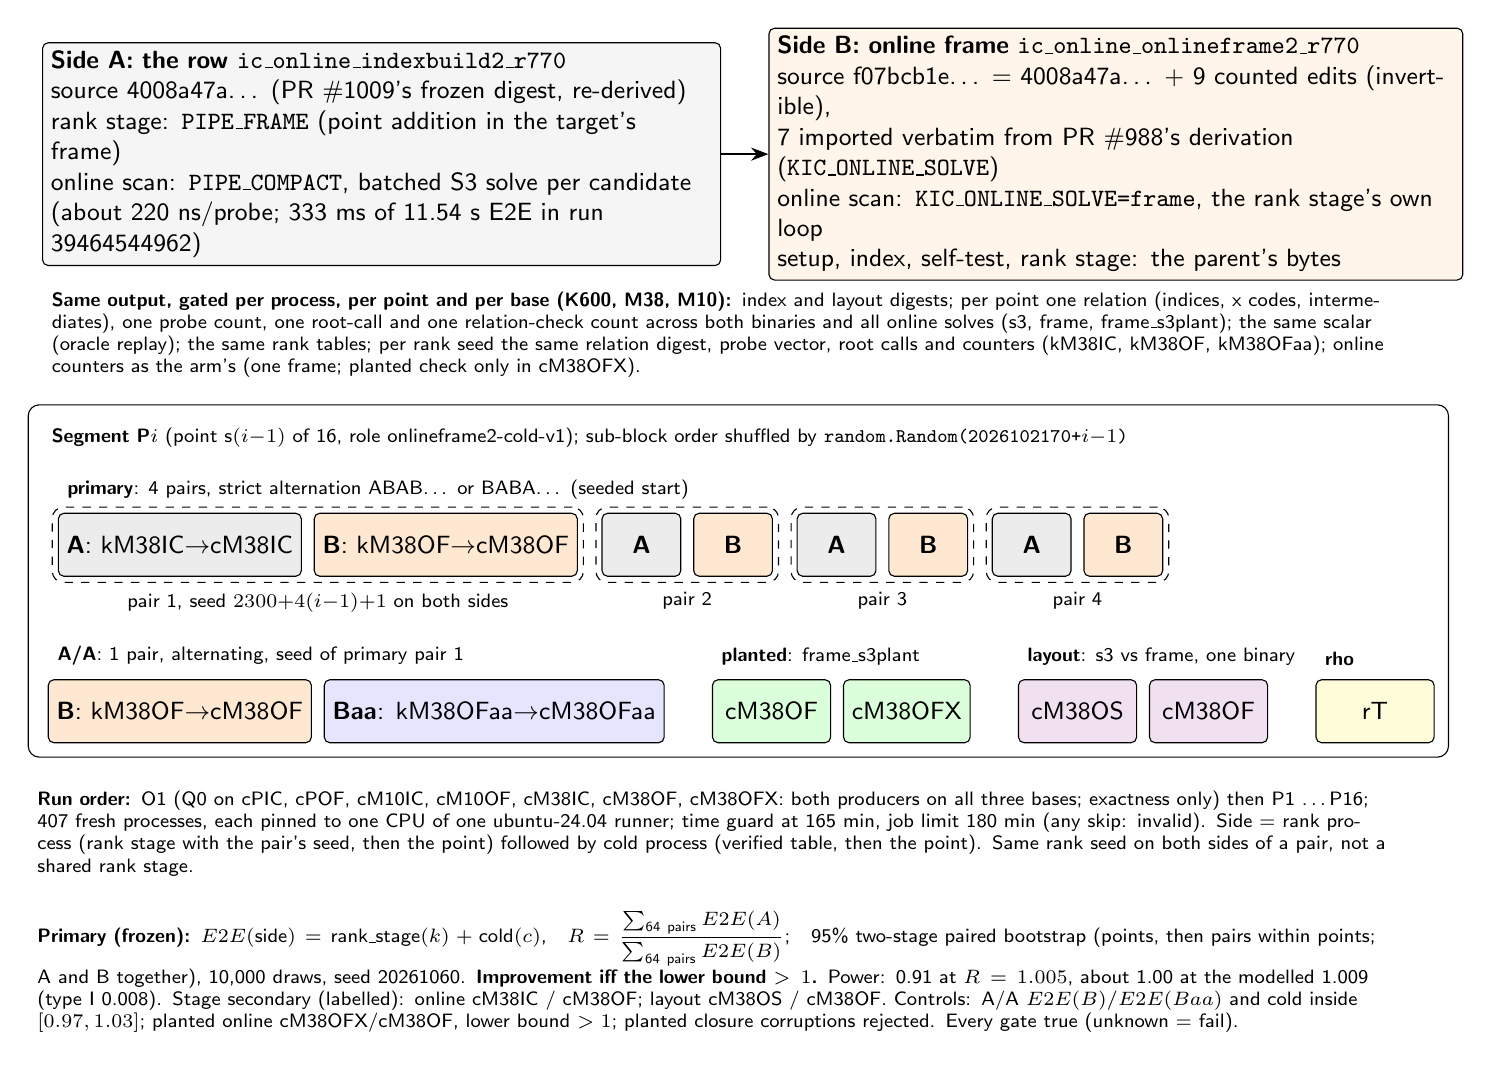
\begin{tikzpicture}[
  font=\sffamily\small,
  box/.style={draw, rounded corners=2pt, align=center, minimum height=8mm, inner sep=3pt},
  sa/.style={box, fill=gray!15, minimum width=24mm},
  sb/.style={box, fill=orange!18, minimum width=24mm},
  sc/.style={box, fill=blue!10, minimum width=24mm},
  sx/.style={box, fill=green!14, minimum width=15mm},
  arr/.style={-{Stealth[length=2.2mm]}, thick},
  note/.style={align=left, font=\sffamily\scriptsize}
]
% producers
\node[box, fill=gray!8, text width=84mm, align=left] (pa) {\textbf{Side A: the row} \texttt{ic\_online\_indexbuild2\_r770}\\
source 4008a47a\ldots\ (PR \#1009's frozen digest, re-derived)\\
rank stage: \texttt{PIPE\_FRAME} (point addition in the target's frame)\\
online scan: \texttt{PIPE\_COMPACT}, batched S3 solve per candidate\\
(about 220 ns/probe; 333 ms of 11.54 s E2E in run 39464544962)};
\node[box, fill=orange!8, text width=86mm, align=left, right=6mm of pa] (pb) {\textbf{Side B: online frame} \texttt{ic\_online\_onlineframe2\_r770}\\
source f07bcb1e\ldots\ = 4008a47a\ldots\ + 9 counted edits (invertible),\\
7 imported verbatim from PR \#988's derivation (\texttt{KIC\_ONLINE\_SOLVE})\\
online scan: \texttt{KIC\_ONLINE\_SOLVE=frame}, the rank stage's own loop\\
setup, index, self-test, rank stage: the parent's bytes};
\draw[arr] (pa.east) -- (pb.west);
\node[note, below=2mm of pa.south west, anchor=north west, text width=172mm] (same) {\textbf{Same output, gated per process, per point and per base (K600, M38, M10):} index and layout digests; per point one relation (indices, x codes, intermediates), one probe count, one root-call and one relation-check count across both binaries and all online solves (s3, frame, frame\_s3plant); the same scalar (oracle replay); the same rank tables; per rank seed the same relation digest, probe vector, root calls and counters (kM38IC, kM38OF, kM38OFaa); online counters as the arm's (one frame; planted check only in cM38OFX).};
% one point segment
\node[note, below=4mm of same.south west, anchor=north west] (ptitle) {\textbf{Segment P$i$} (point s$(i{-}1)$ of 16, role onlineframe2-cold-v1); sub-block order shuffled by \texttt{random.Random(2026102170+$i{-}1$)}};
% primary block
\node[sa, below=7mm of ptitle.south west, anchor=north west, xshift=2mm] (a1) {\textbf{A}: kM38IC$\to$cM38IC};
\node[sb, right=1.5mm of a1] (b1) {\textbf{B}: kM38OF$\to$cM38OF};
\node[sa, right=3mm of b1, minimum width=10mm] (a2) {\textbf{A}};
\node[sb, right=1.5mm of a2, minimum width=10mm] (b2) {\textbf{B}};
\node[sa, right=3mm of b2, minimum width=10mm] (a3) {\textbf{A}};
\node[sb, right=1.5mm of a3, minimum width=10mm] (b3) {\textbf{B}};
\node[sa, right=3mm of b3, minimum width=10mm] (a4) {\textbf{A}};
\node[sb, right=1.5mm of a4, minimum width=10mm] (b4) {\textbf{B}};
\node[draw, dashed, rounded corners, fit=(a1) (b1), inner sep=2pt, label={[note]below:pair 1, seed $2300{+}4(i{-}1){+}1$ on both sides}] {};
\node[draw, dashed, rounded corners, fit=(a2) (b2), inner sep=2pt, label={[note]below:pair 2}] {};
\node[draw, dashed, rounded corners, fit=(a3) (b3), inner sep=2pt, label={[note]below:pair 3}] {};
\node[draw, dashed, rounded corners, fit=(a4) (b4), inner sep=2pt, label={[note]below:pair 4}] {};
\node[note, above=0.5mm of a1.north west, anchor=south west] {\textbf{primary}: 4 pairs, strict alternation ABAB\ldots\ or BABA\ldots\ (seeded start)};
% aa block
\node[sb, below=13mm of a1] (aa1) {\textbf{B}: kM38OF$\to$cM38OF};
\node[sc, right=1.5mm of aa1] (aa2) {\textbf{Baa}: kM38OFaa$\to$cM38OFaa};
\node[note, above=0.5mm of aa1.north west, anchor=south west] {\textbf{A/A}: 1 pair, alternating, seed of primary pair 1};
% planted
\node[sx, right=6mm of aa2] (p1) {cM38OF};
\node[sx, right=1.5mm of p1] (p2) {cM38OFX};
\node[note, above=0.5mm of p1.north west, anchor=south west] {\textbf{planted}: frame\_s3plant};
% layout
\node[sx, right=6mm of p2, fill=violet!12] (l1) {cM38OS};
\node[sx, right=1.5mm of l1, fill=violet!12] (l2) {cM38OF};
\node[note, above=0.5mm of l1.north west, anchor=south west] {\textbf{layout}: s3 vs frame, one binary};
\node[sx, right=6mm of l2, fill=yellow!15] (rt) {rT};
\node[note, above=0.5mm of rt.north west, anchor=south west] {\textbf{rho}};
\node[draw, rounded corners, fit=(ptitle) (a1) (b4) (aa1) (rt), inner sep=5pt] (seg) {};
\node[note, below=3mm of seg.south west, anchor=north west, text width=172mm] (order) {\textbf{Run order:} O1 (Q0 on cPIC, cPOF, cM10IC, cM10OF, cM38IC, cM38OF, cM38OFX: both producers on all three bases; exactness only) then P1 \ldots P16; 407 fresh processes, each pinned to one CPU of one ubuntu-24.04 runner; time guard at 165 min, job limit 180 min (any skip: invalid).
Side = rank process (rank stage with the pair's seed, then the point) followed by cold process (verified table, then the point). Same rank seed on both sides of a pair, not a shared rank stage.};
\node[note, below=2mm of order.south west, anchor=north west, text width=172mm] (prim) {\textbf{Primary (frozen):}
$E2E(\text{side}) = \text{rank\_stage}(k) + \text{cold}(c)$,\quad
$R=\dfrac{\sum_{\text{64 pairs}} E2E(A)}{\sum_{\text{64 pairs}} E2E(B)}$;\quad
95\% two-stage paired bootstrap (points, then pairs within points; A and B together), 10{,}000 draws, seed 20261060.
\textbf{Improvement iff the lower bound $>1$.} Power: 0.91 at $R=1.005$, about 1.00 at the modelled 1.009 (type I 0.008). Stage secondary (labelled): online cM38IC / cM38OF; layout cM38OS / cM38OF. Controls: A/A $E2E(B)/E2E(Baa)$ and cold inside $[0.97,1.03]$; planted online cM38OFX/cM38OF, lower bound $>1$; planted closure corruptions rejected. Every gate true (unknown = fail).};
\end{tikzpicture}
\end{document}
